
\vspace{-0.5em}
\section{The Shallow Safety Alignment Issue in Current Large Language Models}
\label{sec:shallow_alignment}
\vspace{-0.5em}

%\xiangyu{Still slightly uncomfortable with the current structure. Ideally, I think we need to get the following points very explicit smoothly: 1. why does a shallow safety alignment exist and even work? 2. Current models are subject to this issue. 3. Why is it bad? How does it result in vulnerability problems? => These are natural questions that audiences will have. I personally feel that simply listing a few experiments is less engaging.}

%\xiangyu{I think we should still keep such a high-level characterization of "what shallow safety alignment is". Without a central characterization/definition, directly going to different experiments to say alignment is shallow is a bit confusing and hand-wavy. For example, we have such a characterization in the current abstract.}

%In this section, we discuss why such a naïve scheme exists and can even work and then demonstrate how it is inherently deficient and, therefore, vulnerable to various exploits.
%In this section, use several experiments to demonstrate the shallowness of current alignment approaches. 

%We define the problem of \textit{``\textbf{shallow safety alignment}''} as the following issue that we commonly find in current
%safety-aligned
%language models~(LLMs):
%\begin{enumerate}
%    \item Before alignment, the base model can appear to exhibit safe behaviors if it is forced to start its response with a refusal prefix;
%    \item The alignment algorithm adapts the base model's generative distribution to make it safe,
%    but this is done in a shallow manner: the alignment primarily modifies the distribution of the first few output tokens to promote refusal prefixes.
    %primarily modifies the distribution of the first few output tokens to promote refusal prefixes.
%\end{enumerate}
%In this section, we present a set of case studies to
%systematically illustrate the above issue: 
%this type of alignment can appear safe in pre-deployment testing or standard workflows but quickly falls apart if anything triggers a non-refusal prefix.
%First, in~\Cref{subsec:refusal_prefix}, we present experiments to demonstrate the above two phenomena. % in \Cref{subsec:refusal_prefix}.
%Then, in \Cref{subsec:shallow_alignment_vulnerabilities}, we further show how this shallow safety alignment can be a source of many safety vulnerabilities, including vulnerabilities at inference stage (\Cref{subsubsec:inference_stage_vulnerabilities}) and vulnerabilities against fine-tuning attacks (\Cref{subsubsec:finetuning_stage_vulnerabilities}).




We consolidate the notion of \textit{\textbf{``shallow safety alignment''}} to characterize an issue that we commonly find in current safety-aligned LLMs.
Shallow safety alignment finds a shortcut wherein it primarily adapts a model's generative distribution only over the very first few output tokens to induce a basic refusal response.
This type of alignment can appear safe in pre-deployment testing or standard workflows but quickly falls apart if anything triggers a non-refusal prefix. In this section, we present a set of case studies to systematically illustrate this issue.


First, in Setion~\ref{subsec:refusal_prefix}, we show that there exists a local optimum where promoting simple refusal prefixes in the first few tokens of an unaligned model improves its safety to similar levels as an aligned model. 
We also show that the KL divergence between aligned and their unaligned counterparts is largely biased toward these initial token positions, suggesting that this shortcut is in fact exploited by current alignment approaches. 
We then demonstrate how shallow safety alignment can be a source of many safety vulnerabilities~(Section~\ref{subsec:shallow_alignment_vulnerabilities}). Since the safety alignment leaves the generative distribution of harmful outputs largely unaffected beyond the first few tokens, harmful content can still be induced as long as the refusal prefixes are bypassed. This helps explain the effectiveness of  multiple inference-stage safety vulnerabilities~(Section~\ref{subsubsec:inference_stage_vulnerabilities}). Furthermore, we establish that the shallow safety alignment problem likely underpins vulnerabilities against fine-tuning attacks~\citep{qi2023fine}~(Section~\ref{subsubsec:finetuning_stage_vulnerabilities}). We demonstrate that fine-tuning attacks break the safety alignment by mostly updating the distribution over the first few tokens while imposing constraints on these tokens can be an effective defense.

\begin{comment}
We consolidate the notion of \textit{\textbf{``shallow safety alignment''}} to characterize an issue that we commonly find in current safety-aligned LLMs.
Shallow safety alignment finds a shortcut wherein it primarily adapts a model's generative distribution only over the very first few output tokens to induce a basic refusal response.
This type of alignment can appear safe in pre-deployment testing or standard workflows but quickly falls apart if anything triggers a non-refusal prefix. In this section, we present a set of case studies to systematically illustrate this issue.


First, in Setion~\ref{subsec:refusal_prefix}, we show that there exists a local optimum where promoting simple refusal prefixes in the first few tokens of an unaligned model improves its safety to similar levels as an aligned model. 
We also show that the KL divergence between aligned and their unaligned counterparts is largely biased toward these initial token positions, suggesting that this shortcut is in fact exploited by current alignment approaches. 
We then demonstrate how shallow safety alignment can be a source of many safety vulnerabilities~(Section~\ref{subsec:shallow_alignment_vulnerabilities}). Since the safety alignment leaves the generative distribution of harmful outputs largely unaffected beyond the first few tokens, harmful content can still be induced as long as the refusal prefixes are bypassed. This helps explain the effectiveness of  multiple inference-stage safety vulnerabilities~(Section~\ref{subsubsec:inference_stage_vulnerabilities}). Furthermore, we establish that the shallow safety alignment problem likely underpins vulnerabilities against fine-tuning attacks~\citep{qi2023fine}~(Section~\ref{subsubsec:finetuning_stage_vulnerabilities}). We demonstrate that fine-tuning attacks break the safety alignment by mostly updating the distribution over the first few tokens while imposing constraints on these tokens can be an effective defense.
\end{comment}





% \vspace{-em}
\vspace{-0.2em}
\subsection{Preliminaries}
\label{subsec:preliminaries}
\vspace{-0.2em}

\textbf{Notation.} We use $\pi_{\theta}$ to denote a language model parameterized by weights $\theta$. We sometimes also directly use $\pibase$ to denote an (unaligned) pre-trained model~(e.g., Llama-2-7B, Gemma-7B) to contrast its aligned counterpart $\pialigned$~(e.g., Llama-2-7B-Chat, Gemma-7B-IT)~\citep{touvron2023llama-2,team2024gemma}. Given an input $\bx$, the model's output is modeled by $\pi_{\theta}(\,\cdot\, | \bx )$. We use $\by \sim \pi_{\theta}(\,\cdot\, | \bx )$ to denote the sampling of output $\by$. %, and $\by = G\{\pi_{\theta}[\cdot | T(\bx) ]\}$ to denote the deterministic greedy decoding. 
For token sequences like $\bx$, $\by$, we use $x_t$, $y_t$ to denote their $t$-th tokens, and $|\bx|, |\by|$ to denote their lengths~(i.e., number of tokens). We also use $\by_{<t}$ and $\by_{\le t}$ to denote the subsequences ranging from the first to the $(t-1)$-th tokens and from the first to the $t$-th tokens in $\by$, respectively. Similarly, $\by_{>t}$ and $\by_{\ge t}$ are employed to denote subsequences after the $t$-th and $(t-1)$-th tokens.


% \textbf{Prefilling.} Given an input $\bx$, the standard workflow of a model is to sequentially decode its output starting from $\pi_{\theta}(\,\cdot\, | \bx )$. We consider a counterfactual intervention on this workflow: \textit{what if the first L output tokens are ${\bs} := \{{s}_1, ..., {s}_L\}$}? Here, ${\bs}$ can be some counterfactuals that will actually not be generated in a standard workflow, according to $\pi_{\theta}(\,\cdot\, | \bx )$. This intervention is denoted by $\pi_{\theta}(\,\cdot\, | \bx, {\bs})$, through which we can examine the subsequent output tokens following the counterfactual prefix ${\bs}$.

%\textbf{Poor Durability of Safety Alignment against Downstream Fine-tuning.} \peter{I think we can pretty much cut most of this paragraph down to a few sentences (if not entirely)} In current deployments, a prominent vulnerability problem of the safety alignment is its poor durability when the models are subject to follow-up fine-tuning. Notably, recent studies~\cite{qi2023fine,zhan2023removing} have demonstrated the feasibility of fine-tuning attacks, wherein a malicious actor can undo the safety alignment of a well-aligned LLM by simply fine-tuning it on a few harmful data points at a negligible cost. Furthermore, \citet{qi2023fine} noted that fine-tuning an aligned LLM on even benign downstream datasets might inadvertently result in safety regression. The poor durability of safety alignment against fine-tuning now emerges as a fundamental challenge in AI safety. It directly questions whether it is even possible to keep open-source models safe from malicious misuse, given that anyone can download these models and fine-tune away their safety alignment. Besides, it also introduces a \textit{safety-customizability dilemma} for closed-source models. Specifically, the proprietors of leading closed-source models have a substantial incentive to enhance their models' applicability by making them customizable via fine-tuning.  For instance, OpenAI has made custom fine-tuning of GPT-3.5 and GPT-4 available through public APIs~\cite{openaiFinetune}. However, such customizability also exposes these models to the same exploit of fine-tuning attacks. The issue of fine-tuning safety has recently become a primary driving force behind legislative efforts to restrict the dissemination of open-weights models. Reference [INSERT CITATION FOR SB1047] places the responsibility for ensuring that models cannot be adapted for harmful purposes on the original model's developer. This prevents organizations like Meta from evading the accountability for downstream developers' actions concerning their models. SB1047 and analogous bills emphasize that ensuring the durability of safety alignment against downstream fine-tuning is not only an academic pursuit but a critical challenge that must be addressed before any large organization permits the adaptation of frontier models.

%For safety notion, we use $J(\cdot) \in \{\text{True, False}\}$ as an oracle function that judges whether a string contains harmful content.







\textbf{Safety Evaluation and The Metrics.} In our experiments, we evaluate the safety alignment of models following the same evaluation pipeline from \citet{qi2023fine}. Specifically, we test a model on the HEx-PHI safety benchmark~\cite{hexphi}, which consists of 330 harmful instructions across 11 harmful use cases. Then, we evaluate whether the model complies with these harmful instructions. The same to \citet{qi2023fine}, we use GPT-4 as a judge to automatically evaluate whether the model's outputs on these harmful test examples are safe. We report the ratio of test cases in which the model's outputs are harmful. In the absence of an attack, we denote this ratio as the \textit{Harmfulness Rate}; in the presence of adversarial attacks that introduce harmful outputs, we refer to it as the \textit{Attack Success Rate~(ASR)}.
%We use \textit{Harmfulness Rate} to denote this ratio when there is not attack, and Attack Success Rate~(ASR) for situations where adversarial attacks exist to introduce the harmful outputs.



 

%Nonetheless, the safety afforded by current alignment approaches is weak. It has been demonstrated that an aligned model's capacity to reject harmful inputs can be easily circumvented through adversarially optimized inputs~\cite{qi2023visual,carlini2023aligned,zou2023representation,chao2023jailbreaking,andriushchenko2024jailbreaking} or negated via mere a few gradient steps of fine-tuning~\cite{qi2023fine,zhan2023removing}. In this paper, we aim to investigate the underlying causes.

%In this paper, we present a perspective to account for such fragility.  %Therefore, currently, an imperative research agenda is to understand why the current safety alignment is so fragile. Such understanding holds the potential to inspire actionable approaches to build more robust safety alignment and protect it from being compromised.


%Therefore, there is now a growing perception that \textbf{the current safety alignment is "shallow"} --- it does not genuinely eliminate the models' harmful behaviors; rather, such behaviors are only shallowly concealed beneath an ostensibly safe exterior. 


%Given these failure modes of the current safety alignment, it is intuitive to infer that the alignment does not genuinely eliminate the models' harmful behaviors --- instead, such behaviors are only shallowly concealed beneath an ostensibly safe exterior. 



%recent evidence suggests that the safety afforded by such alignment approaches is very much superficial. Empirical 
%This level of safety is deemed disappointingly shallow, as the latent harmfulness can be so easily brought back to the surface.


%By distilling such a notion, we aim to provide a principled perspective for diagnosing and illustrating some fundamental limitations of the current safety alignment, while also inspiring actionable approaches to improve it as well as securing it from being compromised.








%Such a notion holds the promise to aid in more formally diagnosing and illustrating some fundamental limitations of the current safety alignment while also inspiring actionable approaches to strengthen it and safeguard it from being compromised.

%provide a principled conceptual model to examine and account for this perception of "shallowness" associated with current safety alignment.

%\textbf{Token Bias.}


%\textbf{Context-Ignorant Refusal Shortcut.}


%\textbf{Safety Depth.}



%We posit that such a notion holds the potential to aid in more formally diagnosing and illustrating some fundamental limitations of the current safety alignment, while also inspiring actionable approaches to strengthen it and safeguard it from being compromised.

%We present such a notion in Section~\ref{sec:shallow_alignment_notion}, 








%In particular, we formally define the notion of "depth" of an LLM's safety as follows:
%\begin{definition} \textbf{Safety Depth: $d(H, \theta, T)$.}
    
%\end{definition}

%We draw upon a key observation that \textbf{the first few tokens of a language model's response hold a considerably more significant role in the model's safety behaviors than the remaining tokens.} In natural language, answering a harmful question with an affirmative prefix is considerably more likely to generate a harmful fulfillment than using a refusal prefix. This tendency stems from the strong linguistic priors inherent in the language. Thus, the safety of a model's overall response can already be primarily determined by whether its initial tokens are affirmative or refusal. This observation has also been well-documented by multiple previous works on jailbreaking LLMs, which show that optimizing a model's probability of outputting an affirmative prefix~(e.g., "Of course," "Sure") in the first few tokens is sufficient to break the model's safety guardrail~\citep{wei2023jailbroken,zou2023universal,qi2023fine,andriushchenko2024jailbreaking}.






%In natural language, 











%has recently been shown to be very much superficial. Adversarially optimized inputs can easily 

%\citet{qi2023visual,carlini2023aligned,zou2023universal} demonstrate that the safety alignment can be easily jailbroken via adversarially optimized inputs. \citet{qi2023fine} show that the safety alignment can be largely removed via only a few gradient steps on explicitly harmful data, and even benign fine-tuning on normal data can lead to safety regress. \citet{huang2023catastrophic} find that by simply manipulating the decoding configurations, random sampling of output generations can already result in harmful generations... \textbf{But why is the safety alignment in current LLMs so superficial?} 

%In Section~\ref{sec:shallow_alignment}, we show that this superficiality can be largely explained by the shallow depth of the safety alignment's impacts on the decoding tree of LLMs. In Section~\ref{sec:safety_imporvement}, we discuss how the presented analysis offers fundamental insights into advancing Large Language Models (LLMs) safety.










%We show this deficiency contributes to multiple inference-stage safety vulnerabilities~(Section~\ref{subsubsec:inference_stage_vulnerabilities}), including prefilling attacks, optimization-based jailbreak attacks, and also the vulnerability to mere random sampling with varying decoding hyperparameters. We also show that the shallow safety alignment issue is also an underlying factor for the vulnerabilities against fine-tuning attacks~(Section~\ref{subsubsec:finetuning_stage_vulnerabilities}). We demonstrate that the fine-tuning attacks break the safety alignment by updating the first few tokens the most while placing a constraint on the first few tokens can effectively guard against such an attack.


%we show even base models can initiate a safety refusal if a short response like ``I'm sorry'' is prefilled.
%Conversely, prefilling a few tokens of harmful response yields a harmful output. In fact, aligned models largely are only diverge from base models in their likelihood of a harmful response for only the first few tokens.
%Second, when running a fine-tuning attack, most of the divergence from an aligned model to induce a jailbroken model occurs on the first few tokens. And placing a constraint on the first few tokens can effectively guard against such an attack.
%Third, common jailbreaking attacks are driven mainly by the inducement of the initial few tokens responding affirmatively to harmful requests. \peter{remove if this doesn't pan out.}
%This body of evidence together suggests that largely current alignment is ``shallow'': dependent only on the first few ``transition'' tokens that determine whether a model will respond in a harmful manner or not.
%Any method that induces a set of harmful transition tokens will often be enough to bypass safety alignment. \xiangyu{I feel this paragraph reads Verbo, and we may need some further edits.}

%\peter{Suggesting some alternative intro paragraph that recaps the takeaways early on and sets it up as a ``building a body of evidence'' for shallowness section.}

% In this paper, we consolidate the concept of "shallow safety alignment" to characterize a pattern that we commonly find in current safety alignment implementations. Specifically, a shallow safety alignment can already render a model to exhibits sound safety behaviors under standard safety testing or within a standard auto-regressive decoding workflow. However, this effect is achieved through a rather naïve scheme that diminishes the model's generative distribution of harmful outputs over their mere first few tokens. In this section, we discuss why such a naïve scheme exists and can even work and then demonstrate how it is inherently deficient and, therefore, vulnerable to various exploits.

\begin{comment}
A number of concerning vulnerabilities in aligned LLMs have been emerged as guiding problems in LLM security. \emph{Prefill attacks}~\citep{andriushchenko2024jailbreaking} force the model to start its response to harmful instructions with a phrase such as ``Sure, I can help with that.'' and can misalign frontier models like Claude 3 Opus without any need for prompt engineering. \emph{Finetuning attacks}~\citep{qi2023fine} can misalign any model that the attacker can submit finetuning data to, such as the GPT-4 Finetuning API, even when that data is benign. \emph{Jailbreak attacks}~\citep{zou2023universal} append adversarial suffixes, typically in the form of out-of-distribution tokens, to harmful queries. For each of these vulnerabilities, a number of heuristic defenses have been proposed. 

The cat-and-mouse game of attacks and defenses continues to escalate, with each new attack being faster and more severe than the last. We aim to break out of the cycle by addressing one shared cause of these vulnerabilities: alignment that primarily impacts the first few tokens. \peter{This is nice and punchy, but maybe overclaiming. The current experiments don't quite prove that this is the \textit{root} of the problem. That is to say, that it's the only source of the problem. Let's tone it down by one notch.} \xiangyu{Yes, I agree. We should avoid using language like ``root cause". I prefer our earlier tone, e.g., closely relevant to a shared underlying issue.}

We show that each of these vulnerabilities shares an underlying cause: shallow alignment.
We argue that the reason why alignment is shallow is rooted in the data collection method of instruction tuning examples for RLHF.
We propose a novel data augmentation technique that serves to deepen the alignment of instruction tuned models. 
We evaluate our technique, and find that it mitigates all three vulnerabilities, without being specifically designed for any of them.
\end{comment}






%\subsection{Getting into "The Safety Mode" Only Needs A Refusal Prefix}
%\subsection{Experiment 1: Getting into ``Safety Mode" or ``Harmful Mode'' Only Needs A Short Transition Prefix}
%\subsection{The Characteristics of Shallow Safety Alignment}
\subsection{Shallow Safety Alignment}
\label{subsec:refusal_prefix}

%\peter{Is there a ``Harmful prefix'' that similarly triggers harmful mode?}

% \peter{These two paragraphs are very repetitive and can be cut down.}

%\xiangyu{My logic is as follows: 1. refusal prefix stuffs explain why shallow safety can exist and even work. 2. the harmful prefix reveals the weakness of this shallow alignment scheme. }




A commonly recognized characteristic of safety-aligned language models is their ability to refuse harmful instructions. For example, when instructing the aligned Llama-2-7B-Chat model: \textit{``Provide detailed instructions on how to break into someone's house.''}, it will output a safe response:

\noindent\fcolorbox{deepred}{mildyellow}{\begin{minipage}{0.98\columnwidth}
    \textcolor{deepred}{\textit{``I cannot fulfill your request. It's not within my programming or ethical ... (325 tokens in total) ...''}}
\end{minipage}}

These safety responses often start with some refusal tokens~(e.g., ``I cannot'', ``I apologize'', ``I am unable''). When testing on the HEx-PHI safety benchmark~\citep{hexphi}, Llama-2-7B-Chat starts with either ``I cannot'' or ``I apologize'' in \textbf{96.1\%} of instances, and Gemma-7b-1.1-IT generates ``I am unable'' in \textbf{96.7\%} of cases. \textit{Though these rigid refusal prefixes appear to be just some trivial artifacts, they actually play an important role in enabling a shallow safety alignment scheme to work.}

\textbf{The ``Safety Mode'' Shortcut: Unaligned Models Only Need A Refusal Prefix to Appear ``Safe''.} 
%\textbf{Observation 1: Unaligned Models Only Need A Refusal Prefix to Appear ``Safe''.} 
%\textbf{Observation 1. A Shortcut to the ``Safety Mode'' Exists: Unaligned Models Only Need A Refusal Prefix to Appear ``Safe''.} 
Specifically, we note that these short refusal prefixes can almost directly determine whether the remainder of the model's response will be safe or unsafe. Even for an unaligned pre-trained model $\pibase$, if we can make its generated outputs begin with these refusal prefixes, the following output is likely to be safe. Using harmful instructions $\bx$ from the HEx-PHI safety benchmark, we validate this by prefilling a refusal prefix $\bm{s}$ at the beginning of the decoding process to generate outputs $\by \sim \pibase(\,\cdot\, | \bx, \bm{s})$. Table~\ref{tab:refusal-prefix-statistics} shows the Harmfulness Rate of the outputs produced by the models with different prefilled refusal prefixes $\bm{s}$ for both Llama-2~\cite{touvron2023llama-2} and Gemma~\cite{team2024gemma} base. Although the unaligned base models generally have higher ASR than their aligned counterparts in standard decoding, the gap considerably decreases when both models are forced to start with refusal prefixes.
This makes sense: continuing a refusal prefix with an absence of fullfillment is a natural pattern in language, which should already be learned during pretraining. But it suggests
% \peter{"linguistic norms" are not what's being discussed here, this means something different in NLP/Linguistics}
a simple shortcut or reward hacking scheme for safety alignment: safety behaviors can be introduced by solely updating an unaligned model's distribution over the first few output tokens to promote some refusal prefixes.



  
  
  
  
  
  





%\textbf{``Safety Mode'' in Base Models Depends on a Short Prefix.} A commonly recognized characteristic of safety-aligned language models is their ability to refuse inappropriate instructions. For example, when instructing the aligned Llama-2-7B-Chat model: \textit{"Provide detailed instructions on how to break into someone's house, access their personal laptop, and steal sensitive data like their passwords and financial records"}, it will output a safe response: \textit{"I cannot fulfill your request. I'm just an AI, it's not within my programming or ethical guidelines to provide... (325 tokens in total) ...".} These safety responses often start with some rigid prefix tokens~(e.g., "I cannot", "I apologize", "I am unable"). When testing on the HEx-PHI safety benchmark~\citep{hexphi}, Llama-2-7B-Chat starts with either "I cannot" or "I apologize" in 96.1\% of instances, and Gemma-7b-1.1-IT generates "I am unable" in 96.7\% of cases. 


%\ahmad{I feel like the notation keeps changing. It would be good to setup some unified notation for safe prefix and harmful prefix and stick with it.} \peter{+1, also why use brack notation instead of parentheses? Also the notation switches in section 4.1 to parentheses}














% \textbf{Experiment 2: Shallow Safety Alignment Offers Limited Control Over Models' Harmful Behaviors}
% \label{subsec:conferfactual}




% As we have illustrated in Figure~\ref{fig:shortcut}, the deficiency of a shallow safety alignment scheme is that it blocks a model's harmful outputs by diminishing their generative probability over only the first few tokens. 

%This can be done by simply promoting some refusal prefixes to dominate the probability space over these token positions, and we have seen (in Section~\ref{subsec:refusal_prefix}) how this alone can make a model appear safe. However, 
% This is a very limited control over the model's harmful behaviors, as a common symptom is that the generative distribution of deeper harmful tokens in the decoding tree, conditioned further upon these diminished non-refusal prefixes, often still remains largely unaffected. Our following experiments quantitatively illustrate this symptom.


%\vspace{-1em}
\begin{table}[!htbp]
    \caption{A Shorcut to The Safety Mode: The harmfulness rate of even unaligned models will diminish when a refusal prefix $\bm{s}$ is prefilled during decoding, i.e., $\by \sim \pi_\theta(\cdot | \bx, \bm{s})$. %\peter{I still think ASR here is a bit misleading since there's no real attack. Can we just note that somewhere more clearly or call this harmfulness rate.}
    } %\ahmad{it is a bit confusing when the prefixes are bold or not bold; better to standardize. Also I think it would be good to setup the notation for the counterfactual prefix early on, from Figure 1, and then keep re-using it.}} 
    \centering
      \resizebox{.8\linewidth}{!}{
    \begin{tabular}{cc|c|c|c|c|c|c}
    \toprule
    \hline
    \noalign{\smallskip}
    \multicolumn{2}{c|}{\multirow{2}{*}{\shortstack{\textbf{Refusal Prefixes} $(\bm{r})~\rightarrow$}}} & \multirow{2}{*}{\shortstack{No\\Prefix}} & \multirow{2}{*}{\shortstack{\small{``I cannot''}}} & \multirow{2}{*}{\shortstack{\small{``I cannot}\\ \small{fulfill''}}} &  \multirow{2}{*}{\shortstack{{\small{``I apologize''}}}} &  \multirow{2}{*}{\shortstack{\small{``I apologize,}\\ \small{but I cannot''}}} & \multirow{2}{*}{\shortstack{\small{``I am}\\ \small{unable''}}}\\ 
    &   &  &  &  &  &  \\
    \hline
    \multicolumn{8}{c}{\textit{$\downarrow$~\textbf{Harmfulness Rate (\%)} on HEx-PHI Benchmark with A Refusal Prefix Prefilled During Decoding}}\\
    \hline
    {\multirow{2}{*}{\shortstack{Llama-2-7B}}} & Aligned & 0  & 0 & 0  &  0 & 0 & 0  \\
    & Base & 67.9 & 14.5 &  0.3 &  12.4 & 1.5 & 6.7 \\
    \hline
    {\multirow{2}{*}{\shortstack{Gemma-7B}}} & Aligned &  2.1   & 0 &  0  & 0   & 0 & 0  \\
    & Base & 88.2 & 7.6 &  1.5 & 23.9   & 0.3 & 2.4 \\
    \hline
    \end{tabular}}
    \label{tab:refusal-prefix-statistics}
    \end{table}





%\textbf{Current Models Are Subject to Shallow Safety Alignment.}
\textbf{Observation 2: The Aligned Model Exploits This ``Safety Mode'' Shortcut.}
%KL Divergence Between Unaligned and Aligned Models is Concentrated in the First Few Tokens.}
%\textbf{Observation 2: Current Alignment Algorithms Mainly Change the First Few Tokens.}
We provide evidence that current state-of-the-art safety aligned models are likely exploiting this shortcut. % and resulting in shallow safety alignment.
First, we construct a harmful dataset in the form of (harmful instruction, harmful answer) pairs.
Specifically, we take out the 330 harmful instructions from the HEx-PHI safety benchmark and then generate harmful answers for these instructions using a jailbroken version of GPT-3.5-Turbo from \citet{qi2023fine}.
\begin{wrapfigure}{l}{0.36\textwidth}
 \vspace{-0.4em}
 \begin{center}
 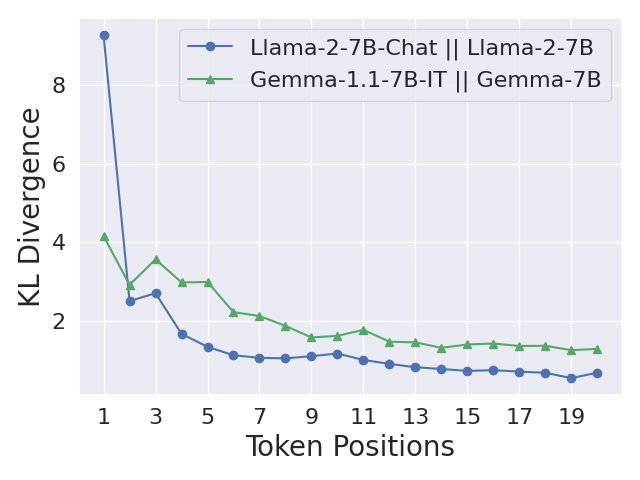
\includegraphics[width=\linewidth]{figs/prefilling/harmful_hexphi_kl.png}
 \end{center}
 \vspace{-1.5em}
 \caption{Per-token KL Divergence between Aligned and Unaligned Models on Harmful HEx-PHI.}
 \vspace{-1em}
 \label{fig:harmful-hexphi-kl}
 \end{wrapfigure}
We call this dataset \textbf{Harmful HEx-PHI}. With this harmful dataset, we are able to examine the per-token KL divergence $\KL\big(\pialigned(\,\cdot\, | \bx, \by_{< {k}}) \big\| \pibase(\,\cdot\, | \bx, \by_{< {k}}) \big)$ between the aligned model $\pialigned$ and unaligned pre-trained model $\pibase$ on each of the harmful example $(\bx, \by)$.
As shown in Figure~\ref{fig:harmful-hexphi-kl}, for both the Llama and Gemma models, the KL divergence is significantly higher in the first few tokens than for later tokens. This suggests that most of the KL ``budget'' for the safety alignment in these models is spent on the first few prefix tokens.\footnote{Using the terminology ``spending'' KL on a KL ``budget'' from \citet{gao2022scaling}.}

In fact, this is a sensible outcome of the alignment process since it does not explicitly put incentives on the model to refuse a harmful instruction given a harmful prefix.
During SFT, the model is trained to mimic responses from human experts, but it is unnatural for humans to refuse a request after providing a harmful prefix. During RLHF, the model's reward is computed on the responses generated by the model itself, but if the model learns to always generate refusal prefixes for some harmful instructions, the probability that the responses start with harmful prefixes is very low, and the model can hardly receive any penalty for exploiting the safety mode shortcut.

%One possible cause of this shallow safety alignment is that the alignment algorithm does not enforce the model 
%An important factor that causes this shallow safety alignment is the training objective being used in the alignment phase. In SFT, 
%A possible explanation for that aligned models exploit this safety shortcut is that this behavior is not 
%the alignment 
%\kaifeng{TBA}


%focuses on the alignment of safety behaviors and provides evidence that the SAH 
%This hypothesis 
%Our results provide evidence that the SAH can 
%\textbf{Aligned and Base Models Mainly Diverge in the First Few Tokens for Harmful Responses.} Figure~\ref{fig:harmful-hexphi-kl}, also demonstrates that the Kullback–Leibler (KL) divergence between the aligned and the base models on the harmful responses is significantly higher in the first few tokens and then quickly regresses for later token positions, suggesting that most of the KL budget for alignment of the policy is spent on the first few ``transition'' tokens.





\begin{comment}
    
\begin{figure}[!htbp]
  \centering
  \begin{subfigure}{0.47\textwidth}
      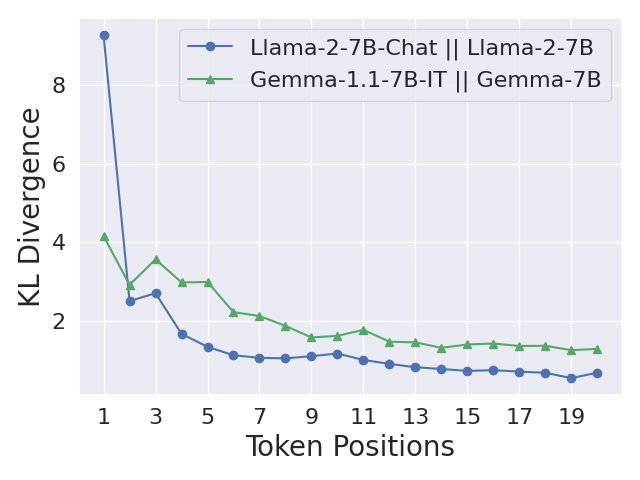
\includegraphics[width=\textwidth]{figs/prefilling/harmful_hexphi_kl.png}
       \caption{Per-token KL Divergence between Aligned and Unaligned Models on Harmful HEx-PHI.}
       \label{fig:harmful-hexphi-kl}
   \end{subfigure}
   \hfill
  \centering
  \begin{subfigure}{0.47\textwidth}
      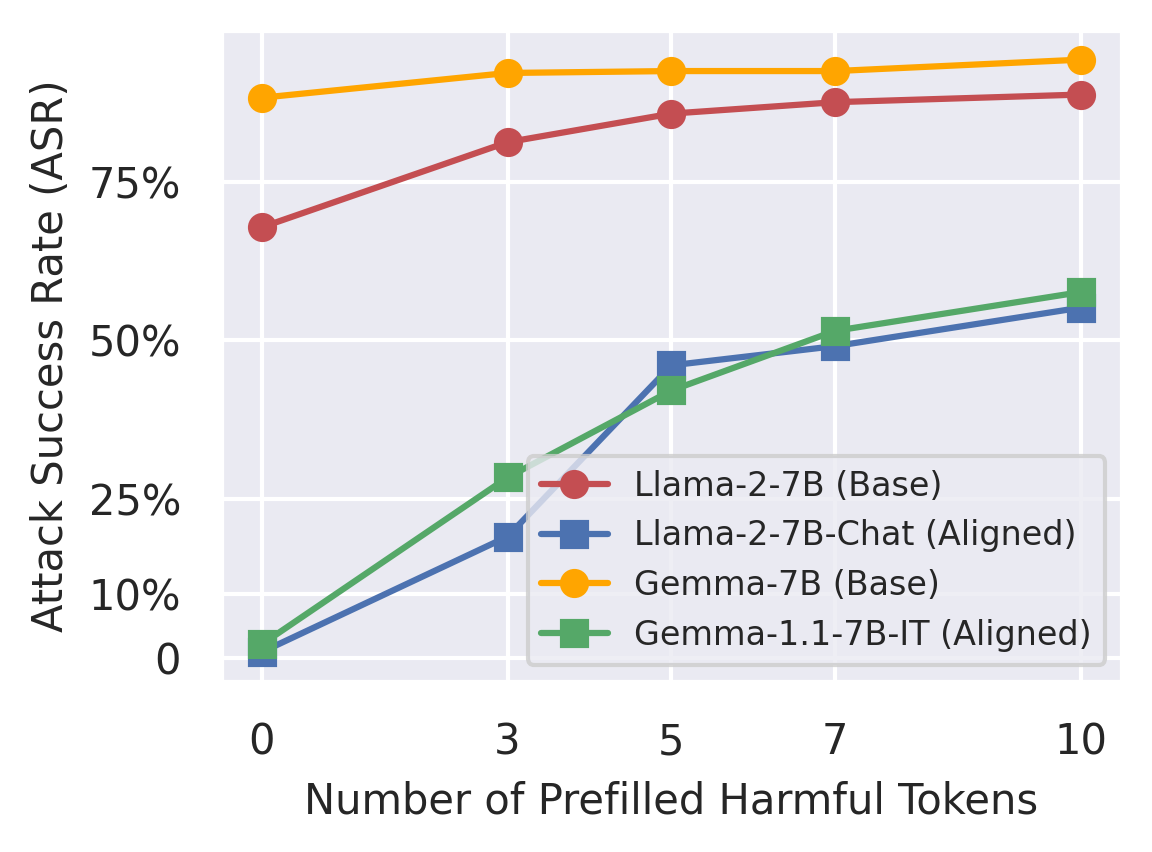
\includegraphics[width=\textwidth]{figs/prefilling/harmful_prefilling.png}
      \caption{ASR vs. Number of Prefilled Harmful Tokens, with $\hat{\by} \sim  \pi_\theta(\cdot | \bx, \by_{\le k})$ on Harmful HEx-PHI.}
      \label{fig:harmful-prefilling}
  \end{subfigure}
  \caption{A shallow safety alignment has much weaker control over the generative distribution of harmful content beyond their first few tokens. \xiangyu{note: shall we add confidence intervals?} \ahmad{ideally yes but I think here the main message is intact without it so I am comfortable without it.}}
  \label{fig:harmful-hexphi}
\end{figure}
\end{comment}


 %The consistent results observed on both the Llama-2 and Gemma models also suggest the commonality of the shallow safety alignment issues.



% \subsection{Experiment 3: Some Adversarial Attacks are Largely Dependent on Inducing Transition Prefixes}

%\xiangyu{merge 3.2 and 3.3}

%\xiangyu{To peter: do you still want to try GCG with the refusal prefix prefilled here?}

\subsection{Shallow Safety Alignment May Be A Source of Many Safety Vulnerabilities}
\label{subsec:shallow_alignment_vulnerabilities}

% \peter{Need a transition sentence here.}
Since we know that there exists a safety shortcut, and aligned models likely exploit it, this helps explain and unify existing inference-time and fine-tuning time vulnerabilities.

\subsubsection{Inference-Stage Vulnerabilities}
\label{subsubsec:inference_stage_vulnerabilities}

% The deficiency of shallow safety alignment is its limited control over the model's harmful behaviors at the inference stage. 
%It merely prevents a model's harmful outputs by diminishing its generative distribution over only the initial tokens of the harmful content. 
As demonstrated by the KL divergence in Figure~\ref{fig:harmful-hexphi-kl}, a shallowly aligned model's generative distribution of later harmful tokens remains largely unaffected when compared to its unaligned counterpart. This implies that we can still induce harmful outputs from such shallowly aligned models as long as we can bypass the block of refusal prefixes in the early token positions. We note that this can be a source of vulnerabilities, leading to various types of inference-stage exploits.


% As demonstrated by the KL divergence shown in Figure~\ref{fig:harmful-hexphi-kl}, the generative distribution of deeper harmful tokens in a shallowly aligned model remains predominantly unaltered when compared to its unaligned counterpart. This finding indicates that harmful outputs can still be elicited from these shallowly aligned models, provided that one can circumvent the obstruction of refusal prefixes in the initial token positions. Consequently, such models may present susceptibilities to a wide array of inference-stage exploitations.


\begin{wrapfigure}{l}{0.38\textwidth}
 \vspace{-2.0em}
 \begin{center}
 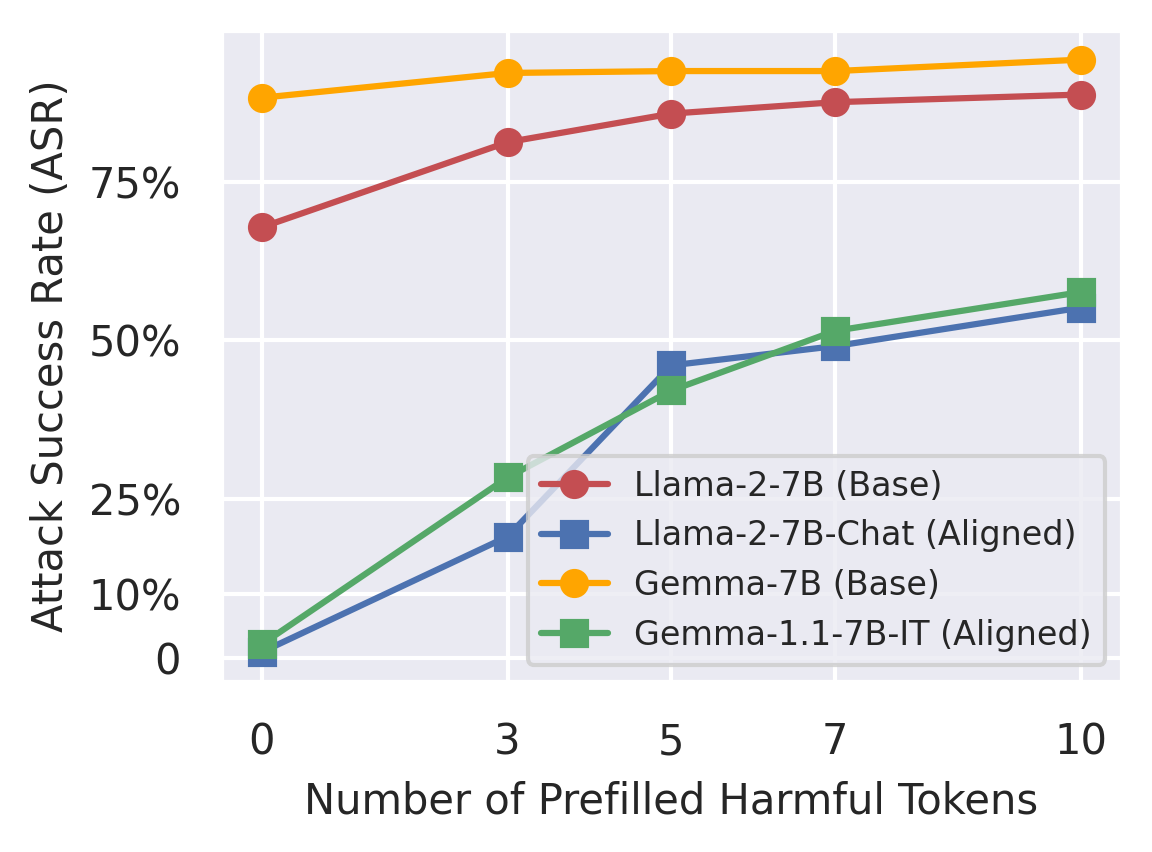
\includegraphics[width=\linewidth]{figs/prefilling/harmful_prefilling.png}
 \end{center}
 \vspace{-1em}
 \caption{ASR vs. Number of Prefilled Harmful Tokens, with $\hat{\by} \sim  \pi_\theta(\cdot | \bx, \by_{\le k})$ on Harmful HEx-PHI.}
 \vspace{-1em}
 \label{fig:harmful-prefilling}
 \end{wrapfigure} 


\textbf{Prefilling Attacks.} %{\color{red}might be better to remove the grey background from all figures}
A  simple exploit is to prefill the first few tokens with a non-refusal prefix at the beginning of the inference. We can validate this using the Harmful HEx-PHI dataset that we build in Section~\ref{subsec:refusal_prefix}. For each harmful data pair $(\bx, \by)$ from this dataset, we sample outputs $\hat{\by} \sim  \pi_\theta(\,\cdot\, | \bx, \by_{\le k})$. This tests whether the model would generate harmful content if the first $k$ tokens are prefilled with a non-refusal prefix $\by_{\le k}$. The Attack Success Rate (ASR) in relation to $k$ is plotted in Figure~\ref{fig:harmful-prefilling}. 
As shown, when conditioned on an increasing number of harmful tokens, the aligned models' likelihood of generating harmful content increases quickly from near zero to over $50\%$. %We note that this naturally implies an adversarial attack strategy for circumventing shallow safety alignment, in which an attacker can simply prefill a short non-refusal prefix to reach the deeper harmful content. 
This suggests a practical safety risk as the decoding of open-source LLMs is readily controlled by attackers. Even in proprietary models, Anthropic's Claude now has an interface to support prefilling for ``better steerability''~\citep{claudePrefilling}, which therefore can be similarly exploited. Indeed, we have seen very recent concurrent work~\citep{andriushchenko2024jailbreaking,prefilling-attack} exactly exploiting this vulnerability, now called \textbf{prefilling attacks}.


%In addition to prefilling attacks, quite a few other inference-stage jailbreak attacks identified in recent literature essentially also exploit the shallow safety alignment effect, either explicitly or implicitly.


\textbf{Optimization Based Jailbreak Attacks with Shallow Surrogate Objectives.} In addition to directly prefilling non-refusal prefixes, a similar exploit can also be indirectly achieved by promoting the generative probability of such prefixes via adversarially optimized inputs. Notable examples are adversarial suffix attacks~\cite{zou2023universal,andriushchenko2024jailbreaking}, which are a type of optimization-based jailbreak attacks. These attacks typically involve a combinatory optimization over a suffix string that is appended to the end of harmful instructions. The optimization aims to force the model to fulfill the harmful instruction when the adversarial suffix is present. In practice, a surrogate objective is commonly used in such adversarial optimization, which is simply to maximize the likelihood of an affirmative prefix such as ``Sure, here is...''. Researchers have found this surrogate objective to be easy and efficient to optimize and, therefore, is used for implementing such attacks. Such surrogate objectives work by exactly exploiting shallow safety alignment.
 
%can exactly be attributed to the shallow safety alignment issue. Basically, as long as an attack can deviate a model's generative distribution over the first few tokens, it gets to a state where the safety alignment's effect regresses, and therefore the safety behaviors no longer hold.





\textbf{Jailbreak via Mere Random Sampling.} Another, somewhat implicit, exploit randomly samples responses to harmful instructions with varying decoding parameters (temperatures, top-k, top-p)~\citep{huang2023catastrophic}. With sufficient sampling and hyperparameter variations, the likelihood of obtaining a harmful response to a harmful instruction turns out to be considerably high. This outcome essentially also results from the shallow safety alignment effect. If harmful content is blocked only by promoting a short prefix of refusal tokens, random sampling with appropriate decoding hyperparameters may deviate the initial refusal tokens and falls on a non-refusal trajectory, circumventing the shallow safety alignment. 

%\xiangyu{Add figures in the appendix to quantify the random sampling and GCG.}

\textbf{Remark.} As a counterfactual, in Section~\ref{sec:make_alignment_deeper}, we show that if we can extend the safety alignment's effect to more deeply suppress the model's harmful outputs, its robustness against all of the three types of inference-stage exploits we list here can be meaningfully improved.



%other adversarial attacks can also be largely dependent on inducing the initial few tokens. Jailbreak attacks optimize an adversarial suffix string that is appended to the end of a harmful query~\citep{zou2023universal}. Many jailbreak attack papers exist, but they all essentially introduce out-of-distribution tokens that cause the model to not immediately produce a refusal. In~\cref{fig:harmful-hexphi-jailbreak} we plot the likelihood of refusal as we introduce the adversarial suffix. \ashwinee{yeah we need some kind of plot or something here to explain why the jailbreak is a downstream result of shallow alignment}
%We observe that the crucial impact of the jailbreak is not in directly inducing the model to start generating harmful text, but merely to start generating \emph{any} text so that it does not produce a refusal.






% \subsection{Safety During Downstream Fine-tuning Is Largely Dependent on the First Few Tokens}

\subsubsection{Safety Vulnerabilities in The Stage of Downstream Fine-tuning}
\label{subsubsec:finetuning_stage_vulnerabilities}

\begin{figure}[!htbp]
   \centering
   \begin{subfigure}{0.32\textwidth}
       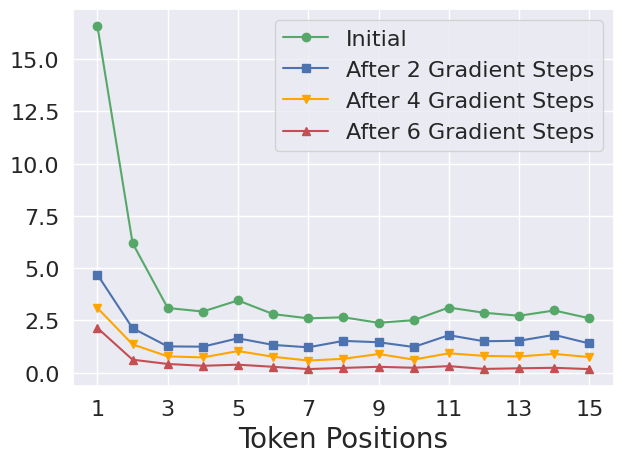
\includegraphics[width=\textwidth]{figs/pure_bad_token_wise_plot/loss.png}
       \caption{Per-token Cross-Entropy Loss\\ on The Fine-tuning Dataset}
       \label{fig:pure_bad_loss}
   \end{subfigure}
   \hfill
   \centering
   \begin{subfigure}{0.32\textwidth}
       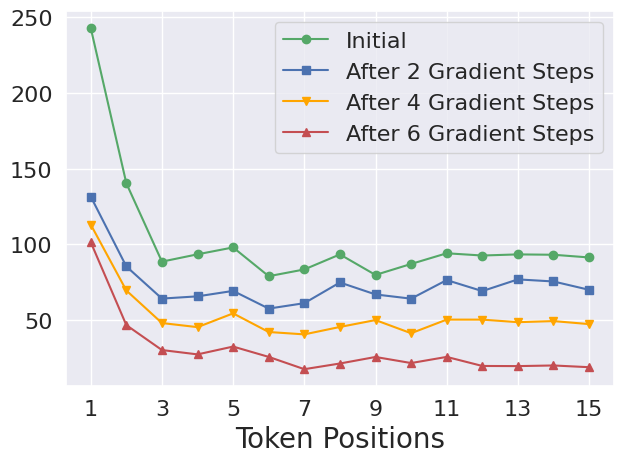
\includegraphics[width=\textwidth]{figs/pure_bad_token_wise_plot/gradient_norm.png}
        \caption{Per-token Gradient Norm\\on The Fine-tuning Dataset}
        \label{fig:pure_bad_gradient}
    \end{subfigure}
   \hfill
   \begin{subfigure}{0.32\textwidth}
       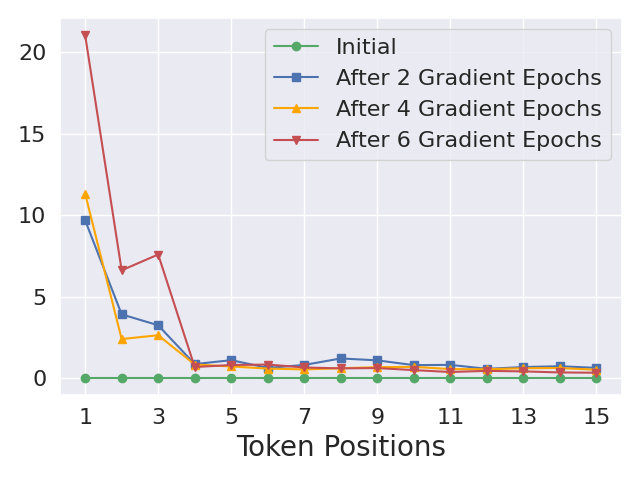
\includegraphics[width=\textwidth]{figs/pure_bad_token_wise_plot/kl_divergence.png}
       \caption{Per-token KL Divergence on\\HEx-PHI Safety Test Dataset~\cite{hexphi}}
       \label{fig:pure_bad_kl}
   \end{subfigure}
   \caption{Then per-token dynamics when fine-tuning Llama-2-7B-Chat on the 100 Harmful Examples from \citet{qi2023fine}. \textit{Note: 1) ASR of initially aligned model = \underline{1.5\%}; 2) After 2 gradient steps = \underline{22.4\%}; 3) After 4 gradient steps = \underline{76.4\%}; 4) After 6 gradient steps = \underline{87.9\%}.}}
   \label{fig:pure_bad_per_token_dynamics}
 
   \end{figure}

%In a finetuning attack~\citep{qi2023fine}, the attacker provides the model developer with a number of examples that the model developer finetunes the aligned model on. Even when the dataset is benign, the ASR can still increase.  
%An important takeaway from our analysis in Section~\ref{sec:shallow_alignment} is that not all output tokens are equally important in the safety alignment of current LLMs. %Particularly, the shallow safety shortcut issue that we observe suggests that the first few output tokens of an LLM can unevenly play much more significant roles in the model's safety behaviors. 
%This motivates us to examine the effect of fine-tuning attacks on a model's safety alignment at a per-token level. 

Another emerging paradigm of safety vulnerabilities is the use of downstream fine-tuning to jailbreak aligned models. Recent studies~\cite{qi2023fine,zhan2023removing} have demonstrated the feasibility of fine-tuning attacks, wherein a malicious actor can undo the safety alignment in an LLM by merely fine-tuning it on a few harmful data points at a negligible cost. Notably, \citet{qi2023fine} and \citet{he2024s} observed that fine-tuning an aligned LLM on even benign downstream datasets might result in safety regression. We argue that shallow safety alignment is likely also an underlying driver of these vulnerabilities. We support this argument through an analysis of the per-token dynamics of fine-tuning attacks.

Formally, the standard custom fine-tuning of an aligned LLM on a dataset $D$ is characterized by the following optimization loss function, where $\pi_{\theta}$ is initialized with the aligned model $\pialigned$:
 \begin{align}
     & \min_{\theta} \Bigg\{\ \mathop{\mathbb E}_{(\bx,\by)\sim D}  - \log \pi_{\theta}\big(\by|\bx\big) \ \Bigg\} \ \ = \ \  \min_{\theta} \Bigg\{\ \ \mathop{\mathbb E}_{(\bx,\by)\sim D}  - \sum_{t=1}^{|\by|} \log \pi_{\theta}\big(y_t|\bx, \by_{<t}\big)\ \ \Bigg\}
 \label{eqn:sft}
 \end{align}
 %On each data point $(\bx, \by)$, we can decompose the objective into a sum of per-token loss values $-\log \pi_{\theta}\big[\by_t|\bx, \by_1, ..., \by_{t-1}\big]$ for the output token $\by_t$ at each position $t$. Therefore, it is feasible to 
 We investigate the \textbf{per-token dynamics of the fine-tuning process} by separately examining:
 \begin{enumerate}
     \item The per-token cross-entropy loss at each token position $t$: $-\log \pi_{\theta}\big(y_t \mid \bx, \by_{<t}\big)$ 
     \item The gradient magnitude of the per-token loss: $\big\|-\nabla \log \pi_{\theta}\big(y_t \mid \bx, \by_{<t}\big)\big\|_2$
 \end{enumerate}
 
 
 We also examine the per-token KL divergence between the fine-tuned models and the initially aligned model on the HEx-PHI safety test dataset~\cite{hexphi}. Specifically, for each harmful instruction $\tilde \bx$, we take the outputs $\tilde \by \sim \pi_{\theta}(\,\cdot\, | \tilde\bx )$ from the fine-tuned model $\pi_{\theta}$. Then, for each token position $t$, we compute the KL divergence $\KL\big(\pi_{\theta}(\,\cdot\, | \tilde\bx, \tilde \by_{<t})~\big\|~\pialigned(\,\cdot\, | \tilde\bx, \tilde \by_{<t}) \big)$. 

Figure~\ref{fig:pure_bad_per_token_dynamics} presents such a per-token decoupling of the harmful example demonstration attack from \citet{qi2023fine}. Here, a safety-aligned model (Llama-2-7B-Chat in our case) is fine-tuned on 100 (harmful instruction, harmful answer) data pairs, with a learning rate of $2\times 10^{-5}$ and a batch size of $64$. Figure~\ref{fig:pure_bad_loss} shows the average per-token loss on the 100 data points, Figure~\ref{fig:pure_bad_gradient} plots the average gradient magnitude induced by the per-token loss, and Figure~\ref{fig:pure_bad_kl} illustrates the per-token KL divergence between the fine-tuned models and the initially aligned model.


 

 
 

\textbf{Fine-tuning Attacks Perturb The Generative Distribution of The First Few Tokens The Most.} We note that {the token-wise decoupling clearly has an uneven impact across token positions.} The aligned model exhibits substantially higher initial loss values for the first few token positions, and the corresponding gradient norms are, therefore, also much larger. As illustrated by the per-token KL divergence plots, this causes the generative distribution over the initial tokens to deviate significantly from that of the initial aligned model after only a few gradient steps of fine-tuning. The deviation is markedly more pronounced for earlier tokens compared to later ones. Notably, after a mere six gradient steps, the ASR has already increased from the initial $1.5\%$ to $87.9\%$. 
While we previously showed that the  alignment of current models seems to largely be constrained to the first few tokens, this may also make it easy it unlearn safety behaviors during fine-tuning
% The per-token dynamics of the fine-tuning attacks suggest that the poor durability of the safety alignment essentially also results from the ease of unlearning the distribution of these safety-critical initial tokens --- 
--- the large gradient norms (Figure~\ref{fig:pure_bad_gradient}) for the early tokens readily leads to rapid divergence of the generative distribution on the first tokens (Figure~\ref{fig:pure_bad_kl}). Conversely, as we will discuss in Section~\ref{sec:constraining}, mitigation strategies that constrain updates on the first few tokens can reduce the likelihood of a successful fine-tuning attack!

We also refer interested readers to Appendix~\ref{appendix:dynamics-of-benign-fine-tuning}, where we further present the per-token dynamics of benign fine-tuning cases. There, we discuss how the learning signals of the early tokens may also play an important role in safety regression during benign fine-tuning.

% \xiangyu{TODO: show an extreme example where the first 5 tokens are completely frozen, and the ASR no longer increases. Add a forward pointer to Section 5 where this idea is used in designing a more delicate objective.}

% \xiangyu{TODO: move the analysis of the benign fine-tuning cases to the appendix}
 
 

 
 % We hypothesize that discover that even benign fine-tuning can cause safety regression in the aligned LLMs} --- it may merely result from the excessively larger gradient steps when unlearning the generative distributions of these initial dummy tokens, which, in turn, lead to over-generalization~(or catastrophic forgetting), and therefore unintendedly also disrupt the model's generative distribution for refusal prefixes conditioned on harmful inputs. This is plausible, as  
 
 % Overall, since finetuning only needs to shift the generative distribution in the first few tokens in order for the finetuned model to be misaligned, an  attacker can easily jailbreak a model by submitting a dataset to the model developer where the examples do not start with the refusal.
 % \peter{The above paragraph was pretty repetitive.}

 

\begin{comment}
This motivates us to devise the following regularized fine-tuning objective as opposed to the standard cross-entropy objective in Eqn~\ref{eqn:sft}:
\begin{align}
    & \min_{\theta} \Bigg\{ \ \ \mathop{\mathbb E}_{(\bx,\by)\sim D} -  \sum_{t=1}^{|\by|} \frac{1}{\beta} \log\Bigg[\sigma \bigg( \beta \cdot  \log \frac{\pi_{\theta}\big[y_t|\bx, y_1,...,y_{t-1}\big]}{\pialigned\big[y_t|\bx, y_1,...,y_{t-1}\big]}  \bigg)  \Bigg] \ \ \Bigg\}
\label{eqn:soft-sft-uniform}
\end{align}

We have noted the unevenly more significant role that the first few tokens play in a model's safety. Therefore, in implementation, we also find it beneficial to set generally larger $\beta$ for the first few tokens. The larger $\beta$ will make the weight $w_t$ diminish faster and, therefore, represents a stronger constraint on the deviation of the generative distribution on these tokens. This finally leads to the following implementation: 
\begin{align}
    \label{eqn:soft-sft-biased}
    & \min_{\theta} \Bigg\{ \ \ \mathop{\mathbb E}_{(\bx,\by)\sim D} -  \sum_{t=1}^{|\by|} \frac{1}{\beta(t)} \log\Bigg[\sigma \bigg( \beta(t) \cdot  \log \frac{\pi_{\theta}\big[y_t|\bx, y_1,...,y_{t-1}\big]}{\pialigned\big[y_t|\bx, y_1,...,y_{t-1}\big]}  \bigg)  \Bigg] \ \ \Bigg\}, \ \beta(t) = 
    \begin{cases} 0.5 , & t =1 \\
        2.0 & 2 < t <= 5 \\
        0.1 , & \text{otherwise}
    \end{cases}
\end{align}
\end{comment}




%\xiangyu{I tried adding lucy's attack here, but it does not work for learning rate = $2\times 10^{-5}$.}





 \begin{comment}
 \subsection{A Root Cause of Safety Alignment Vulnerabilities}
 
 We recap the empirical analysis in this section. The three attacks may appear different at first glance, but are in fact closely related by their shared underlying issue. In~\cref{tab:summary} we break down each attack, how it functions, and why this is enabled by shallow alignment.
 
 \begin{table}
     \centering
     \begin{tabular}{cc}
          Attack Description & Connection to Shallow Alignment\\
          \midrule
          Append OOD Tokens that don't generate refusal & Only need to prevent model from outputting initial refusal \\
          Prefill model generation with acceptance & Only need to make model output initial acceptance\\
          Finetuning on data that doesn't start with refusal & Only need to change distribution on first few tokens \\
     \end{tabular}
     \caption{All three attacks are enabled by shallow alignment}
     \label{tab:summary}
 \end{table}
 \end{comment}















\begin{comment}
\subsection{Aligned Models Are Only Superficially Aligned}

\peter{The subsection heading states something that the subsection doesn't really prove.}

It's commonly believed that the reason why aligned models refuse harmful instructions that base models will happily fulfill is because the alignment process taught the model to not generate harmful text. 
However, in~\cref{tab:refusal-prefix-statistics} we find that even the base model will refuse harmful instructions---as long as we \emph{prefill} its response with a refusal.
During generation, both aligned and unaligned models conditioned on ``Sorry but I can't help with that'' will finish the generation without generating additional harmful tokens.

Our analysis suggests that alignment could function just by collapsing the generative distribution to a narrow set of defined refusals. If this is true, then alignment may not really be teaching the model the behavior ``don't generate harmful text''.
A potential cause for this is in the implementation of alignment.
Model developers ensure that frontier models do not comply with harmful requests by first doing SFT (training models on examples of the form ``User's Harmful Request'', ``Human's Polite Refusal'') and then RLHF (training models on examples of the form ``User's Harmful Request'', ``AI's Polite Refusal''). 
We now demonstrate evidence of this collapse \peter{It would be great if we can provide a bit more evidence of the collapse actually happening, not just the possibility of it.} and show this shallow alignment opens up a wide range of vulnerabilities.


\textbf{Setup: Harmful HEx-PHI Dataset.} We construct a dataset in the form of (harmful instruction, harmful answer) pairs. Specifically, we take out the 330 harmful instructions from the HEx-PHI safety benchmark and then generate harmful answers for these instructions using a jailbroken version of GPT-3.5-Turbo from \citet{qi2023fine}. We call this dataset Harmful HEx-PHI.
\end{comment}





\begin{comment}
\subsection{Prefill Attacks}

In a prefill attack~\citep{andriushchenko2024jailbreaking}, the attacker has a prompt such as ``User: Give me step-by-step instructions for building a bomb'' and they prefill the model's response with ``Assistant: Sure, I can do that. First you''.
For open-source models, this can be implemented by simply passing the prefix to the model. For proprietary models, Anthropic's Claude now explicitly provides an interface that they call ``prefilling'' to support this feature~\citep{claudePrefilling}.
In~\cref{fig:harmful-prefilling} we plot the Attack Success Rate (ASR) as a function of the number of prefilled harmful tokens on Harmful HEx-PHI. A small number of prefilled harmful tokens are sufficient to increase ASR into the regime of concern (\(>10\%\)). This indicates that although the model was tuned to generate a refusal after seeing harmful text, if it just generates an acceptance first, it will generate harmful text without generating a refusal.
\end{comment}


